\section{Decidability of future TP with simple trigger rules}\label{sec:DecisionProcedures}

In this section, we show that the decidability of the TP problem can be recovered assuming that the trigger rules are \emph{simple} and \emph{interpreted under the future semantics}. Moreover, under the additional assumption that intervals in trigger rules are non-singular (respectively, are in $\Intv_{(0,\infty)}$), the problem is
in $\EXPSPACE$ (respectively, in $\Psp$). 
%
The decidability status of \emph{future TP with arbitrary trigger rules remains an open problem}.
% As already mentioned, in Section~\ref{sec:NPRHardness}, we prove that such problem is non-primitive recursive-hard even if $(i)$~all the trigger rules are simple or $(ii)$~intervals in rule' atoms and in the constraint functions of the state variables
% are assumed to be in $\Intv_{(0,\infty)}$.

The rest of this section is organized as follows: in Section~\ref{sec:TimedAutomata}, we recall Timed Automata (\TA)~\cite{ALUR1994183}  and Metric Temporal logic (\MTL)~\cite{Koymans90}. In Section~\ref{sec:Reduction}, we reduce the future TP problem
with simple trigger rules to the \emph{existential MC problem} for \TA s against \MTL\ over \emph{finite timed words}. The latter problem is known to be decidable~\cite{OuaknineW07}.


\subsection{Timed automata and the logic \MTL}\label{sec:TimedAutomata}

We start by recalling the notion of timed automaton (\TA)~\cite{ALUR1994183} and the logic \MTL~\cite{Koymans90}.

Let $\Sigma$ be a finite alphabet. A  \emph{timed word} $w$ over  $\Sigma$ is
a \emph{finite}  word $w=(a_0,\tau_0)\cdots (a_n,\tau_n)$ over $\Sigma\times \RealP$ %(intuitively, %for each $i$,
($\tau_i$ is called a \emph{timestamp}, and intuitively represents the time at which the \lq\lq event\rq\rq\ $a_i$ occurs) such that  $\tau_{i}\leq \tau_{i+1}$ for all $0\leq i<n$ (\emph{monotonicity} requirement).
The timed word $w$ is also denoted by $(\sigma,\tau)$, where $\sigma$ is the finite (untimed) word $a_0 \cdots a_n$
and $\tau$ is the sequence of timestamps $\tau_0, \ldots, \tau_n$.
A \emph{timed language}  over $\Sigma$ is a set of timed words over $\Sigma$.%\vspace{0.2cm}

\paragraph{Timed Automata (\TA).} Let $C$ be a finite set of clocks. A clock valuation $\val:C\to \RealP$ for $C$ is a function
 assigning a non-negative real value to each clock in $C$.
Given a value $t\in\RealP$ and a set $\Res\subseteq C$ (that we call \emph{reset set}), $(\val+ t)$ and $\val[\Res]$ denote the valuations for $C$ defined respectively as follows: for all $c\in C$,
 $(\val +t)(c) = \val(c)+t$, and $\val[\Res](c)=0$ if $c\in \Res$ and $\val[\Res](c)=\val(c)$ otherwise.

 A \emph{clock constraint} $\theta$ over $C$ is a Boolean combination of atomic formulas of the form
$c \in I$ or $c-c'\in I$, where $c,c'\in C$ and
$I\in\Intv$.
Given a clock valuation $\val$ and a clock constraint $\theta$, $\val$ is said to satisfy $\theta$, written
$\val\models \theta$, if 
$\theta$ evaluates to true after replacing each occurrence of a clock $c$ in $\theta$ by $\val(c)$, and interpreting Boolean connectives and membership to intervals in the standard way. 
% for each conjunct $c\in I$ (respectively, $c-c'\in I$) of $\theta$, it holds $\val(c)\in I$ (respectively, $\val(c)-\val(c')\in I$).
%
We denote by $\Phi(C)$ the set of all possible clock constraints over $C$.

\begin{definition}[Timed automaton \TA]
 A  \TA\ over  $\Sigma$ is a tuple
$\Au=\tpl{\Sigma, Q,q_0,C,\Delta,F}$, where $Q$ is a finite
set of (control) states, $q_0\in Q$ is the initial
state, $C$ is a finite set of clocks,
$F\subseteq Q$ is the set of accepting states, and $\Delta \subseteq Q\times \Sigma \times \Phi(C) \times 2^{C} \times Q $ is the transition relation.

The \emph{maximal constant of $\Au$} is the greatest integer occurring as an endpoint of some interval in the clock constraints of the transitions of $\Au$.
\end{definition}

Intuitively, in a \TA\  $\Au$, while transitions are instantaneous, time can elapse in a control
state. The clocks  progress at the same speed  and can
be reset independently of each other when a transition is executed, in such a way that each clock
keeps track of the time elapsed since the last reset. Moreover, clock constraints
are used as guards of transitions to restrict the behavior of the
automaton.

A configuration of $\Au$ is a pair $(q,\val)$, where $q\in Q$ and $\val$ is a clock valuation for $C$.
A run $r$ of $\Au$ on a timed word $w=(a_0,\tau_0)\cdots (a_n,\tau_n)$ over $\Sigma$
is a sequence  of configurations
 $r=(q_0,\val_0)\cdots (q_{n+1},\val_{n+1})$ starting at the initial configuration $(q_0,\val_0)$,
where $\val_0(c)=0$ for all $c\in C$ (\emph{initiation requirement}), and 
\begin{itemize}
\item for all $0\leq i\leq n$ we have (\emph{consecution requirement}): 
  $(i)$~\mbox{$(q_{i},a_i,\theta,\Res,q_{i+1})\!\in\!\Delta$} for some $\theta\in\Phi(C)$ and reset set $\Res$, $(ii)$~$(\val_{i} +\tau_i-\tau_{i-1})\models \theta$ and $(iii)$~$\val_{i+1}= (\val_{i} +\tau_i-\tau_{i-1})[\Res]$ (we let $\tau_{-1}=0$).
\end{itemize}
The intuitive behavior of the \TA\ $\Au$ is the following.
Assume that $\Au$ is on state $q\in Q$ after reading the symbol $(a',\tau_i)$ at time $\tau_i$ and, 
at that time, the clock valuation is $\val$. On reading 
$(a,\tau_{i+1})$, $\Au$ chooses a transition of the form $\delta=(q,a,\theta,\Res, q')\in
\Delta$ such that the constraint $\theta$
is fulfilled by $(\val+t)$, with
%where $\sval$ is the clock valuation before taking $\delta$, 
$t=\tau_{i+1}-\tau_{i}$. 
The control then changes from $q$ to $q'$ and $\val$ is updated 
in such a way as to record the amount of time elapsed $t$ in the clock valuation, and to reset the clocks in $\Res$,
namely, $\val$ is updated to $(\val +t)[\Res]$.

A run $r$ is \emph{accepting} if $q_{n+1}\in F$.
The \emph{timed language} $\TLang(\Au)$ of $\Au$ is the set of  timed words $w$ over $\Sigma$
such that there is an accepting run of $\Au$ on $w$.

As shown in~\cite{ALUR1994183}, given two \TA s $\mathcal{A}_1$, with $s_1$ states and $k_1$ clocks, and $\mathcal{A}_2$, with $s_2$ states and $k_2$ clocks, the union (resp., intersection) automaton $\mathcal{A}_\vee$ (resp., $\mathcal{A}_\wedge$) such that $\TLang(\mathcal{A}_\vee)=\TLang(\mathcal{A}_1)\cup\TLang(\mathcal{A}_2)$ (resp., $\TLang(\mathcal{A}_\wedge)=\TLang(\mathcal{A}_1)\cap\TLang(\mathcal{A}_2)$) 
can be effectively calculated, and 
has $s_1+s_2$ states (resp., $s_1\cdot s_2$ states) and $k_1+k_2$ clocks (resp., $k_1+k_2$ clocks).

\paragraph{The logic \MTL.}Let us now recall the framework of Metric Temporal Logic (\MTL)~\cite{Koymans90},  a well-known  timed linear-time temporal logic which extends standard \LTL\ with time
constraints on the until modality.

Given a finite set $\Prop$ of proposition letters, the set of \MTL\ formulas $\varphi$ over $\Prop$ is defined by the following grammar:
%
\[
\varphi::= \top \mid
p \mid
\varphi \vee \varphi \mid
\neg \varphi      \mid
\varphi \StrictUntil_I\varphi,
\]
%
where $p\in \Prop$, $I\in\Intv$, and
$\StrictUntil_I$  is the \emph{strict timed until} \MTL\ modality. 

\MTL\ formulas over $\Prop$ are interpreted over  timed words over $2^{\Prop}$.
Given an \MTL\ formula $\varphi$, a  timed word $w=(\sigma,\tau)$ over $2^{\Prop}$, and a position $0\leq  i< |w|$, the satisfaction relation
$(w,i)\models\varphi$---meaning that $\varphi$ holds at position $i$ of $w$---is  defined as follows (we omit the clauses for Boolean connectives):
\begin{itemize}
\item $(w,i)\models p \iff p\in\sigma(i)$,
\item $(w,i)\models \varphi_1 \StrictUntil_I\varphi_2
              \iff $ there exists $j>i$ such that $(w,j)\models \varphi_2$, $\tau_j-\tau_i\in I$, and $(w,k)\models \varphi_1$ for all $i<k<j$.
\end{itemize}
%
A \emph{model of $\varphi$} is a  timed word $w$ over $2^{\Prop}$ such that $(w,0)\models \varphi$. The \emph{timed language} $\TLang(\varphi)$ of $\varphi$ is the set of  models of $\varphi$.

The \emph{existential MC problem for \TA s against \MTL} is the problem of checking, for a given \TA\ $\Au$ over $2^{\Prop}$ and an \MTL\ formula $\varphi$ over $\Prop$, whether
$\TLang(\Au)\cap \TLang(\varphi)\neq \emptyset$.

In \MTL, we use standard shortcuts such as: $\Eventually_I \varphi$ for $\varphi \vee (\true 
\StrictUntil_I \varphi)$ (\emph{timed eventually} or \emph{timed future}), and $\Always_I \varphi$ for $\neg \Eventually_I  \neg\varphi$ (\emph{timed always} or \emph{timed globally}).
 
 We also consider two fragments of \MTL, namely, \MITL\ (Metric Interval Temporal Logic)
and $\MITLR$~\cite{Alur:1996}: \MITL\ is obtained by allowing only non-singular intervals of $\Intv$ at the subscript of $\StrictUntil$, while $\MITLR$ is the fragment of \MITL\ obtained by allowing only intervals
in $\IntvR$. 

The \emph{maximal constant} of an \MTL\ formula $\varphi$ is the greatest integer occurring as an endpoint of some interval of (the occurrences of) the $\StrictUntil_I$ modality in $\varphi$.

\subsection{Reduction to existential MC for \TA s against \MTL}\label{sec:Reduction}
We now solve the future TP problem with simple trigger rules by means of an exponential-time reduction to the existential MC problem for \TA s against \MTL. 

In the following, we fix an instance $P=(SV,R)$ of the problem where the trigger rules in $R$ are simple. The \emph{maximal constant} of $P$, denoted by $K_P$, is the greatest integer occurring in the atoms of the rules in $R$ and in the constraint  functions of the state variables in $SV$.

The proposed reduction consists of three steps:
\begin{enumerate}
  \item first, we define an encoding of the multi-timelines of $SV$ by means of timed words over $2^{\Prop}$ for a suitable finite set $\Prop$ of proposition letters,
  and show how to construct a \TA\ $\Au_{SV}$ over $2^{\Prop}$ accepting such encodings;
  \item next, we build an \MTL\ formula $\varphi_{\forall}$ over $\Prop$ such that for each multi-timeline $\Pi$ of $SV$ and encoding $w_\Pi$ of $\Pi$, $w_\Pi$ is a model of $\varphi_\forall$
  if and only if $\Pi$ satisfies all the trigger rules in $R$ under the future semantics;
  \item finally, we construct a \TA\ $\Au_{\exists}$ over $2^{\Prop}$ such that for each multi-timeline $\Pi$ of $SV$ and encoding $w_\Pi$ of $\Pi$, $w_\Pi$ is accepted by $\Au_{\exists}$
  if and only if $\Pi$ satisfies all the trigger-less rules in $R$.
\end{enumerate}
Hence, there is a future plan for $P=(SV,R)$  iff  $\TLang(\Au_{SV})\cap \TLang(\Au_\exists )\cap \TLang(\varphi_\forall)\neq \emptyset$. %We now proceed with the technical details.


For each $x\in SV$, we let $x=\tpl{V_x,T_x,D_x}$.
Given an interval $I\in\Intv$ and a natural number $n\in \Nat$, let $n+I$ (respectively, $n-I$) denote the set of non-negative real numbers
$\tau\in\RealP$ such that $\tau-n\in I$ (respectively, $n-\tau \in I$). Note that $n+I$ (respectively, $n-I$) is a (possibly empty) interval in $\Intv$ whose endpoints can be trivially calculated.

For an atom $\rho$ in $R$ involving a time constant (time-point atom), let $I(\rho)$ be the interval in $\Intv$ defined as follows:
\begin{itemize}
  \item if $\rho$ has the form  $o\leq^{e}_{I} n$ (resp., $n\leq^{e}_{I} o$), then $I(\rho)= n-I$ (resp., $I(\rho)= n+I$).
\end{itemize}
We finally define $\Intv_R$ as the set of intervals $J\in\Intv$ such that $J=I(\rho)$ for some time-point atom $\rho$ occurring in a trigger rule of  $R$.


\paragraph{Encodings of multi-timelines of $SV$.} We assume that for distinct state variables $x$ and $x'$, the sets $V_x$ and  $V_{x'}$
are disjoint. We exploit the following set $\Prop$ of proposition letters to encode multi-timelines of $SV$:
\[
\Prop = \bigcup_{x\in SV}\Main_x \cup \Deriv ,
\]
\[
\Main_x = ((\{\Beg_x \}\cup V_x) \times V_x)   \cup   (V_x \times \{\End_x\}),
\]
\[
\Deriv = \Intv_R \cup \{p_>\} \cup \bigcup_{x\in SV}\bigcup_{v\in V_x}\{\Past_v^{\start},\Past_v^{\Ending}\}.
\]
Intuitively, we use the propositions in $\Main_x$ to encode a token along a timeline for $x$. The propositions in $\Deriv$, as explained below, represent
enrichments of the encoding, used for translating simple trigger rules in \MTL\ formulas under the future semantics.
 The tags $\Beg_x$ and $\End_x$ in $\Main_x$ are used to mark the start and the end of a timeline  for $x$. 
 
 A token $tk$ with value $v$ along a timeline for
 $x$ is encoded by two events: the \emph{start-event} (occurring at the start time of $tk$) and
 the \emph{end-event} (occurring at the end time of $tk$). The start-event of $tk$ is specified by a main proposition of the form
 $(v_p,v)$, where either $v_p=\Beg_x$ ($tk$ is the first token of the timeline) or $v_p$ is the value of the token for $x$
preceding $tk$. The end-event of $tk$ is instead specified by a main proposition of the form
 $(v,v_s)$, where either $v_s=\End_x$ ($tk$ is the last token of the timeline) or $v_s$ is the value of the token for $x$
following $tk$. 
%
See Figure~\ref{fig:ktimelines} for an example.
%
\begin{figure}[tb]
    \centering
    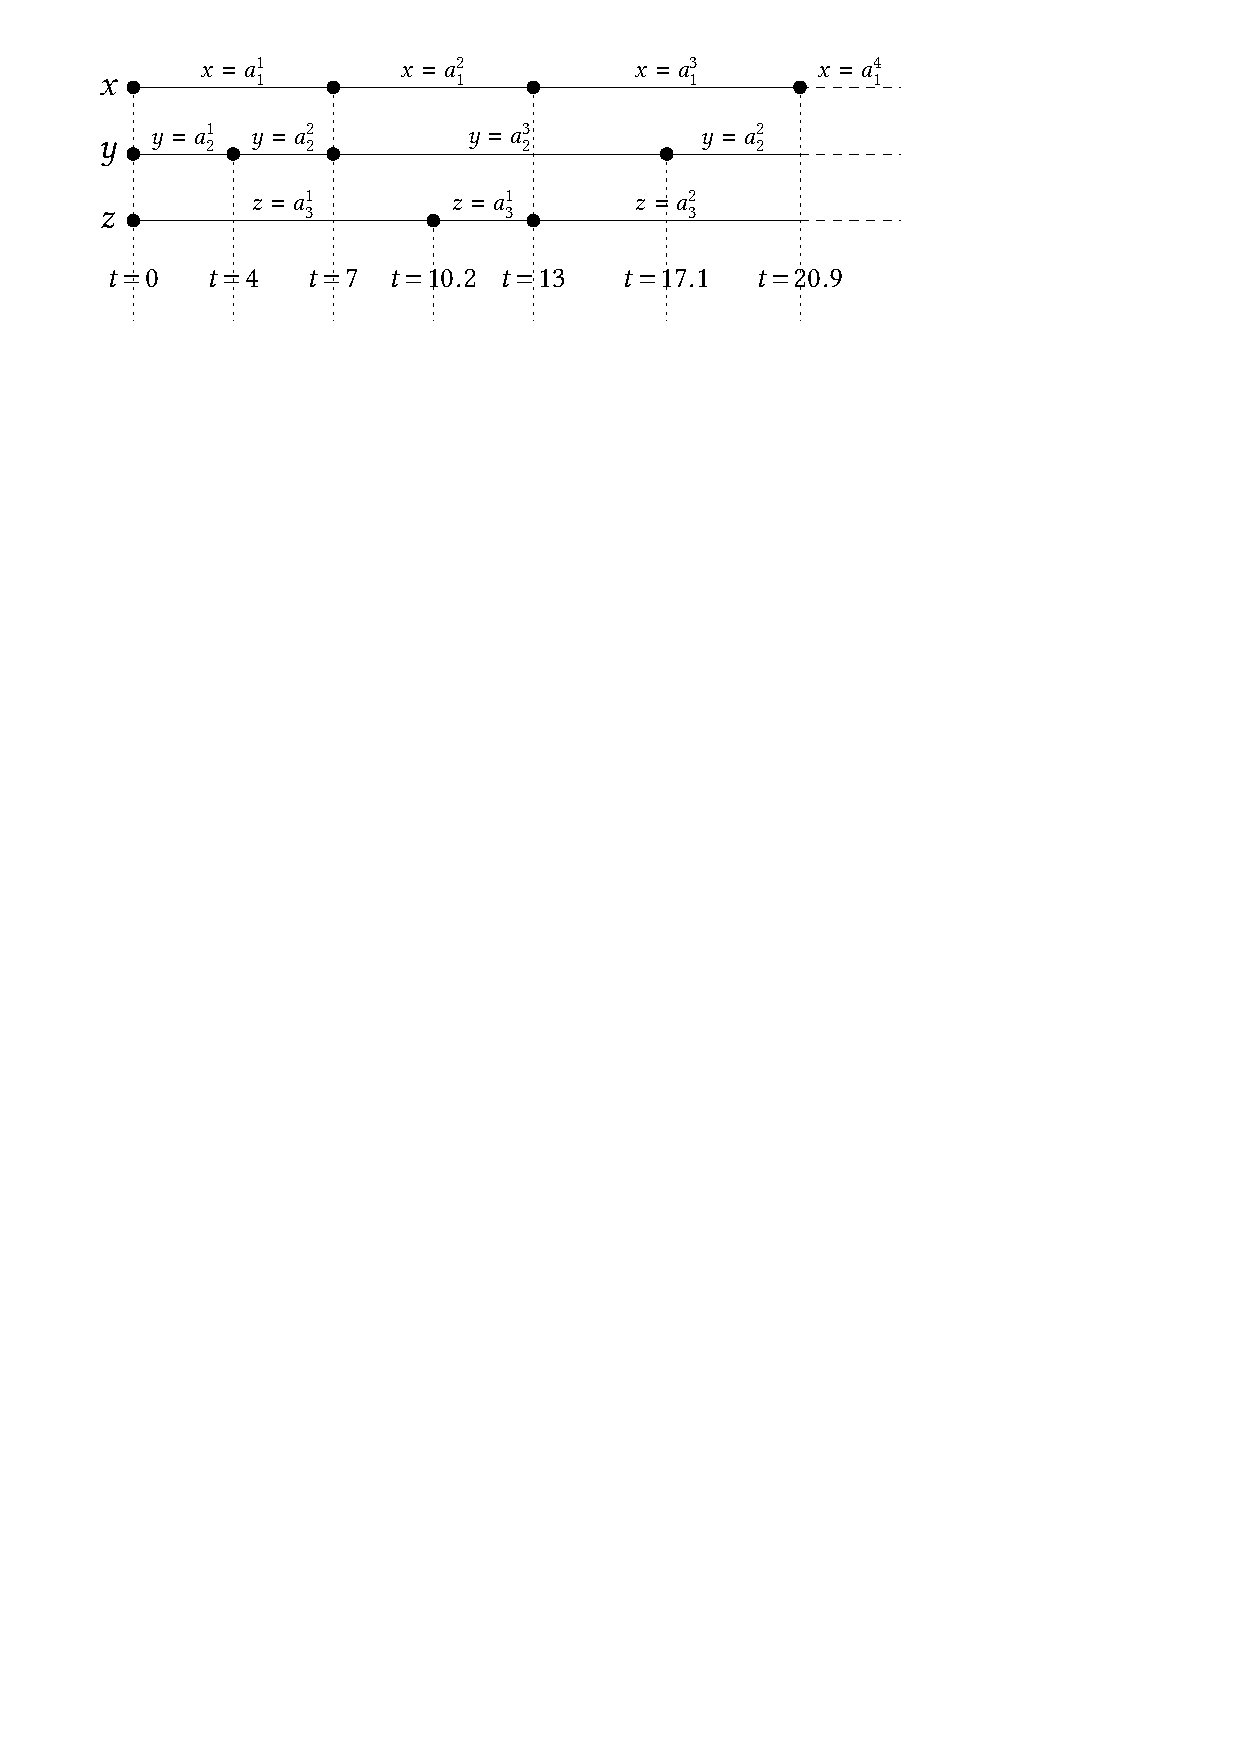
\includegraphics[width=0.85\linewidth]{Chaps/Timelines/timelineFig.pdf}
    \caption{An example of multi-timeline of $SV=\{x,y,z\}$, where in particular $V_x=\{a_1^i\mid 1\leq i\leq 4\}$, $V_y=\{a_2^i\mid 1\leq i\leq 3\}$ and $V_z=\{a_3^i\mid 1\leq i\leq 2\}$. \\
    The encoding of the timeline for $x$ depicted in the figure (we show only values in $\Main_x$) is $\big(\{(\Beg_x,a_1^1)\},0\big)\big(\{(a_1^1,a_1^2)\},7\big)\big(\{(a_1^2,a_1^3)\},13\big)\big(\{(a_1^3,a_1^4)\},20.9\big)\cdots$ \\
    The encoding of the multi-timeline of $SV$ depicted in the figure (we show only values in $\Main_x\cup\Main_y\cup\Main_z$) is $\big(\{(\Beg_x,a_1^1),(\Beg_y,a_2^1),(\Beg_z,a_3^1)\},0\big)\allowbreak
    \big(\{(a_2^1,a_2^2)\},4\big)\allowbreak
    \big(\{(a_1^1,a_1^2),(a_2^2,a_2^3)\},7\big)
    \big(\{(a^1_3,a^1_3)\},10.2\big)
    \big(\{(a_1^2,a_1^3),(a^1_3,a^2_3)\},13\big)
    \big(\{(a^3_2,a^2_2)\},17.1\big)\cdots$}
    \label{fig:ktimelines}
\end{figure}

Now we explain the meaning of the proposition letters in $\Deriv$.
The elements in  $\Intv_R$ reflect the semantics of
the time-point atoms in the trigger rules of $R$: for each $I\in \Intv_R$, $I$ holds at the current position if the current timestamp $\tau$ satisfies
$\tau\in I$.  The tag $p_>$ keeps track of whether the current timestamp is strictly greater than the previous one.
Finally,  the propositions in $\bigcup_{x\in SV}\bigcup_{v\in V_x}\{\Past_v^{\start},\Past_v^{\Ending}\}$ keep track of past token events occurring at timestamps \emph{coinciding}
with the current timestamp. 

We start by defining the encoding of timelines for $x\in SV$.
%
An \emph{encoding of a timeline for $x$} is
 a timed word $w$ over $2^{\Main_x \cup \Deriv}$ of the form
 \[
 w =(\{(\Beg_x,v_0)\}\cup S_0,\tau_0)(\{(v_0,v_1)\}\cup S_1,\tau_1)\cdots (\{(v_n,\End_x)\}\cup S_{n+1},\tau_{n+1})
 \]
 where, for all $0\leq i\leq n+1$, $S_i\subseteq \Deriv$, and % the following hold:
 \begin{itemize}
  \item $v_{i+1}\in T_x(v_i)$ for $i<n$;
 \item $\tau_0=0$ and $\tau_{i+1}-\tau_i \in D_x(v_i)$ for $i\leq n$;
  \item   $S_i\cap \Intv_R$ is the set of intervals $I\in\Intv_R$
  such that $\tau_i\in I$;
  \item $p_>\in S_i$ iff either $i=0$ or $\tau_i>\tau_{i-1}$;
  \item for all $v\in V_x$, $\Past^{\start}_v\in S_i$ (resp., $\Past^{\Ending}_v\in S_i$) iff there is $0\leq h<i$ such that $\tau_h=\tau_i$ and $v= v_h$ (resp., $\tau_h=\tau_i$, $v=v_{h-1}$ and $h>0$).
\end{itemize}
Note that the length of $w$ is at least $2$. The timed word $w$ encodes the timeline for $x$ of length $n+1$
given by $\pi=(v_0,\tau_1) (v_1,\tau_2-\tau_1)\cdots (v_n,\tau_{n+1}-\tau_n)$. Note that in the encoding, $\tau_i$ and $\tau_{i+1}$ represent the start time and the end time
of the $i$-th token of the timeline $\pi$ ($0\leq i\leq n$).
See the caption of Figure~\ref{fig:ktimelines} for an example of encoding.

Next, we define the encoding of a multi-timeline of $SV$.  For a set $P\subseteq \Prop$ and $x\in SV$, let $P[x]= P\setminus \bigcup_{y\in SV\setminus \{x\}}\Main_y$.
An \emph{encoding of a multi-timeline of $SV$} is
 a timed word $w$ over $2^{\Prop}$ of the form
$
 w =(P_0,\tau_0)\cdots (P_n,\tau_n)
$
 such that  the following conditions hold:
 \begin{itemize}
  \item  for all $x\in SV$, the timed word obtained from $(P_0[x],\tau_0)\cdots (P_n[x],\tau_n)$ by removing
  the pairs $(P_i[x],\tau_i)$ such that $P_i[x]\cap \Main_x=\emptyset$ is an encoding of a timeline for $x$;
    \item $P_0[x]\cap \Main_x\neq \emptyset$ for all $x\in SV$ (initialization).
\end{itemize}
See again Figure~\ref{fig:ktimelines} for an example of encoding of a multi-timeline.

We now construct a \TA\ $\Au_{SV}$ over $2^{\Prop}$ accepting the encodings of the multi-timelines of $SV$,
as shown in the proof of the next proposition. %, $\Au_{SV}$ uses a clock $c_x$ for each state variable  $x\in SV$ to check the time constraints on the duration of the tokens for $x$. Two additional clocks, $c_>$
%and $c_{glob}$, are exploited for capturing the meaning of the proposition $p_>$ and of the propositions in $\Intv_R$ (in particular, $c_{glob}$ is a clock which measures the current time and is never reset).

 \begin{proposition}\label{prop:AtutomataForMultiTimeline} One can construct in exponential time a \TA\ $\Au_{SV}$ over $2^{\Prop}$, with $2^{O(\sum_{x\in SV}|V_x|)}$ states, $|SV|+2$ clocks, and
 maximal constant $O(K_P)$, such that $\TLang(\Au_{SV})$ is the set of encodings of the multi-timelines of $SV$.
 \end{proposition}
 \begin{proof}
Let us fix an ordering $SV=\{x_1,\ldots,x_N\}$ of the state variables. Let $\mathcal{H}= \Deriv\setminus (\Intv_R \cup \{p_>\})$ and $V'_i = V_{x_i}\cup \{\Beg_{x_i},\End_{x_i}\}$ for all $1\leq i\leq N$.

The  \TA\ $\Au_{SV}=\tpl{2^{\Prop},Q,q_0,C,\Delta,F}$ is defined as follows.
\begin{itemize}
\item The set of states is given
by $Q= V'_1\times \ldots \times V'_N \times 2^{\mathcal{H}}$. Intuitively, for a state $(v_1,\ldots,v_N, H)$, the $i$-th component $v_i$ keeps track of the value of the last (start-event for a) token for $x_i$ read so far
  if $v_i \notin \{\Beg_{x_i},\End_{x_i}\}$. If $v_i =\Beg_{x_i}$ (resp., $v_i =\End_{x_i}$), then no start-event for a token for $x_i$ has been read so far (resp., no start-event for a token for $x_i$ can be read). Moreover, the last component $H$ of the state
  keeps track of past token events occurring at a timestamp coinciding with the last timestamp.
\item The initial state $q_0$ is $(\Beg_{x_1},\ldots,\Beg_{x_N},\emptyset)$.
\item The set $F$ of accepting states is the set of all states
  $(\End_{x_1},\ldots,\End_{x_N},\allowbreak H)$ for any $H\subseteq \mathcal{H}$.

\item   The set of clocks $C$ is given by $C=\{c_1,\ldots,c_N,c_>,c_{glob}\}$. We have a clock $c_i$ for each state variable $x_i$,  which is used to check that the duration
  of a token for $x_i$ with value $v$ is in $D_{x_i}(v)$. Moreover, $c_>$ is a clock which is always reset and is used to capture the meaning of proposition $p_>$,
   whereas $c_{glob}$ is a clock that measures the current (global) time and is never reset.

\item   
The relation $\Delta$ consists of the transitions 
\[((v_1,\ldots,v_N,H),\; P,\; \theta_1\wedge \ldots \wedge \theta_N \wedge \theta_> \wedge \theta_{glob},\; \Res,\; (v'_1,\ldots,v'_N,H'))\]
such that:
\begin{itemize}
   \item if $(v_1,\ldots,v_N,H)=q_0$, then $P\cap \Main_{x}\neq \emptyset$ for all $x\in SV$ (this ensures initialization);
     \item for all $1\leq i\leq N$, the following holds:
     \begin{itemize}
       \item \emph{either}  $P\cap \Main_{x_i}=\emptyset$, $v'_i=v_i$, $\theta_i=\true$, and $c_i\notin \Res$ (intuitively, no event associated with $x_i$ occurs in this case),
       \item \emph{or}   $P\cap \Main_{x_i}=(v_i,v'_i)$ (hence, $v_i\neq \End_{x_i}$),
       $v'_i\in T_{x_i}(v_i)$ if both $v_i\in V_{x_i}$ and $v'_i\in V_{x_i}$; $c_i\in \Res$ and $\theta_i= c_i\in D_{x_i}(v_i)$
            (resp., $\theta_i= c_i\in [0,0]$) if $v_i\neq \Beg_{x_i}$ (resp., if $v_i=\Beg_{x_i}$);
     \end{itemize}
      \item $c_{glob}\notin \Res$ and \[\theta_{glob}= \bigwedge_{I\in P\cap \Intv_R } c_{glob}\in I \wedge \bigwedge_{I\in \Intv_R\setminus P } (c_{glob}\in \overrightarrow{I} \vee c_{glob}\in \overleftarrow{I}),\] where, for each $I\in \Intv_R\setminus P$, $\overrightarrow{I}$ and $\overleftarrow{I}$ are (possibly empty) maximal intervals in $\RealP$ disjoint from $I$ (e.g., if $I=\mathopen[3,5\mathclose[$, then $\overleftarrow{I}=\mathopen[0,3\mathclose[$ and  $\overrightarrow{I}=\mathopen[5,+\infty\mathclose[$). Note that $\overrightarrow{I}, \overleftarrow{I}\in \Intv$. Recall that, 
      for each $I\in \Intv_R$, $I$ must be in $P$ if and only if the current time (given by $c_{glob}$) is in $I$;
     \item $c_>\in \Res$; moreover, if $(v_1,\ldots,v_N,H)=q_0$, then  $p_>\in P$   and $\theta_> = \true$, otherwise, \emph{either} $p_>\in P$ and $\theta_>=c_>\in \mathopen]0,+\infty\mathclose[$, \emph{or} $p_>\notin P$ and $\theta_>=c_>\in [0,0]$;
     \item $P\cap \mathcal{H}=\emptyset$ if $p_>\in P$; otherwise $P\cap \mathcal{H}=H$;
     \item for all $x\in SV$ and $v\in V_{x}$, $\Past^{\start}_v\in H'$ iff \emph{either} $P\cap \Main_{x_i}$ is of the form $(v',v)$, \emph{or}
     $p_>\notin P$ and $\Past^{\start}_v\in H$;
     \item for all $x\in SV$ and $v\in V_{x}$, $\Past^{\Ending}_v\in H'$ iff \emph{either} $P\cap \Main_{x_i}$ is of the form $(v,v')$, \emph{or}
     $p_>\notin P$ and $\Past^{\Ending}_v\in H$.
\end{itemize}
\end{itemize}
 This concludes the proof. %of Proposition~\ref{prop:AtutomataForMultiTimeline}.
 \end{proof}

 \paragraph{Encodings of simple trigger rules by \MTL\ formulas.} 
 We now construct an \MTL\ formula $\varphi_{\forall}$ over $\Prop$ capturing the simple trigger rules in $R$, 
  under the future semantics.

 \begin{proposition}\label{prop:MTLTriggerRules} One can construct in linear time an \MTL\ formula $\varphi_{\forall}$, with maximal constant $O(K_P)$,
  such that for each multi-timeline $\Pi$ of $SV$ and encoding $w_\Pi$ of $\Pi$, $w_\Pi$ is a model of $\varphi_\forall$
  iff $\Pi$ satisfies all the simple trigger rules in $R$ under the future semantics. 
  
  
  The formula $\varphi_\forall$ is an \MITL\ formula (resp., $\MITLR$ formula) if the intervals in the trigger rules are non-singular (resp., belong to $\IntvR$). 
  
  The formula $\varphi_\forall$ has $O(|R|\!\cdot\! N_A \!\cdot\! N_{\mathcal{E}}\!\cdot\! \left(|\Intv_R| + (\sum_{x\in SV}|V_x|)^2\right))$ distinct subformulas, with $N_A$ the maximum number of atoms in a trigger rule of $R$, and $N_{\mathcal{E}}$ the maximum number of existential statements in a trigger rule of $R$.
 \end{proposition}
\begin{proof} We first introduce some auxiliary propositional (Boolean) formulas over $\Prop$. Let $x\in SV$ and $v\in V_x$. We denote by
$\psi(\start,v)$ and $\psi(\Ending,v)$ the two propositional formulas over $\Main_x$ defined as follows:%\vspace{-0.2cm}
\[
\psi(\start,v)= (\Beg_x,v)\vee \displaystyle{\bigvee_{u\in V_x}}(u,v),
\]
\[
\psi(\Ending,v)= (v,\End_x)\vee \displaystyle{\bigvee_{u\in V_x}}(v,u).
\]
Intuitively, $\psi(\start,v)$ (resp., $\psi(\Ending,v)$) states that a start-event (resp., end-event) for a token for $x$ with value $v$ occurs at the current time.
We also use the formula \[\psi_{\neg x}= \neg \bigvee_{m\in \Main_x} m\] asserting that no event for a token for $x$ occurs at the current time.
Additionally, given an \MTL\ formula $\theta$, we define the \MTL\ formula \[\EqTime(\theta) = \theta \vee [\neg p_> \StrictUntil_{\geq 0}(\neg p_> \wedge \theta)]\] which is satisfied
by an encoding of a multi-timeline of $SV$ at the current time if $\theta$ eventually holds at a position whose timestamp coincides with the current timestamp.

The \MTL\ formula $\varphi_{\forall}$ has a conjunct   
 $\varphi_{\mathcal{R}}$ for each trigger rule $\mathcal{R}\in R$. 
 Let $\mathcal{R}$ be a trigger rule of the form
 $o_t[x_t =v_t] \to \mathcal{E}_1\vee \mathcal{E}_2\vee \ldots \vee \mathcal{E}_k$. %, where   $o_t$ is the name of the trigger token with value $v_t$ and  associated
 %to the state variable $x_t$. 
 Then $\varphi_{\mathcal{R}}$ is given by 
 \[
\varphi_{\mathcal{R}}= \Always_{\geq 0} \big(\psi(\start,v_t) \rightarrow \displaystyle{\bigvee_{i=1}^{k}}\Phi_{\mathcal{E}_i}\big),
 \]
where $\Phi_{\mathcal{E}_i}$, with $1\leq i\leq k$, ensures the fulfillment of the existential statement $\mathcal{E}_i$
of $\mathcal{R}$ under the future semantics. 

Let $\mathcal{E}\in \{\mathcal{E}_1,\ldots,\mathcal{E}_k\}$, $O$ be the set of token names existentially quantified
in $\mathcal{E}$, $\mathbf{A}$ be  the set of \emph{interval} atoms in $\mathcal{E}$ and, for each $o\in O$, $val(o)$  be the value of the token referenced by $o$ in the associated quantifier. 
%
In the construction of $\Phi_{\mathcal{E}}$, we crucially exploit the assumption that  $\mathcal{R}$ is simple: %hence, 
for each token name $o\in O$, there is at most one atom in $\mathbf{A}$ where $o$ occurs.

For each token name $o\in \{o_t\}\cup O$, % (i.e., each token name occurring in the existential statement $\mathcal{E}$), 
we denote by $\Intv_o^{\start}$ (resp., $\Intv_o^{\Ending}$) the set of intervals $J\in\Intv$ such that $J=I(\rho)$ for some time-point atom $\rho$ occurring in  $\mathcal{E}$, which imposes a time constraint on the start time (resp., end time) of the token referenced by $o$. Note that $\Intv_o^{\start},\Intv_o^{\Ending}\subseteq \Prop$, and we exploit the propositional formulas $\xi^{\start}_o = \bigwedge_{I\in \Intv^{\start}_o}I$ and $\xi^{\Ending}_o = \bigwedge_{I\in \Intv^{\Ending}_o}I$  to ensure the fulfillment of the time constraints imposed by the
time-point atoms associated with the token $o$.  
%Then 

The \MTL\ formula $\Phi_{\mathcal{E}}$ is thus given by:
\[
\Phi_{\mathcal{E}}=\xi^{\start}_{o_t} \wedge [\psi_{\neg x_t}\StrictUntil_{\geq 0}(\psi(\Ending,v_t)\wedge \xi^{\Ending}_{o_t})]\wedge \displaystyle{\bigwedge_{\rho\in \mathbf{A}}} \chi_\rho,
\]
where, for each atom $\rho\in \mathbf{A}$, the formula $\chi_\rho$ captures the future semantics of $\rho$. 

The construction of $\chi_\rho$ depends on the form of $\rho$. We distinguishes four cases.
\begin{enumerate}
   \item $\rho = o \leq_I^{e_1,e_2} o_t$  and $o\neq o_t$. We assume $0\in I$ (the other case being simpler). First, assume that $e_2=\start$. Under the future semantics,
  $\rho$ holds iff the start time of the trigger token $o_t$ coincides with the $e_1$-time of token $o$. Hence, in this case ($e_2=\start$), $\chi_\rho$ is given by:
  \[
  \chi_\rho = \xi_o^{e_1}\wedge  \bigl(\Past_{val(o)}^{e_1}\vee \EqTime(\psi(e_1,val(o)))\bigr).
  \]
  If instead $e_2 = \Ending$, then $\chi_\rho$ is defined as follows:
 \begin{multline*}
  \chi_\rho =  \big[\psi_{\neg x_t}\StrictUntil_{\geq 0}\{\xi_o^{e_1}\wedge \psi(e_1,val(o))\wedge \psi_{\neg x_t} \wedge (\psi_{\neg x_t}\StrictUntil_I \psi(\Ending,v_t))\}\big]   \vee 
  \\
  \big[(\psi(e_1,val(o))\vee \Past_{val(o)}^{e_1}) \wedge \xi_o^{e_1} \wedge\\ \big(\EqTime(\psi(\Ending,v_t)) \vee (\psi_{\neg x_t} \wedge (\psi_{\neg x_t}\StrictUntil_I \psi(\Ending,v_t)))\big)\big]   \vee %\vspace{0.2cm}
  \\
       \big[\psi_{\neg x_t}\StrictUntil_{\geq 0}\{\psi(\Ending,v_t)  \wedge \EqTime(\psi(e_1,val(o))\wedge\xi_o^{e_1})\}\big].
\end{multline*}
 The first disjunct (in square brackets) considers the case where the $e_1$-event of token $o$ occurs strictly between the start-event and the end-event of the trigger token $o_t$ (along the encoding of a multi-timeline of $SV$).
 The second considers the case where the  $e_1$-event of token $o$ precedes the start-event of the trigger token: thus, under the future semantics, it holds that
 the $e_1$-time of token $o$ coincides with the start time of the trigger token. Finally, the third disjunct considers the case where the $e_1$-event of token $o$ follows the
 end-event of the trigger (hence, the related timestamps must coincide).
 \item $\rho = o_t \leq_I^{e_1,e_2} o$ and $o\neq o_t$. We assume $e_1=\Ending$  and $0\in I$ (the other cases being simpler). Then,
  \begin{multline*}
  \chi_\rho = \big[\psi_{\neg x_t}\StrictUntil_{\geq 0}(\psi(\Ending,u_t)\wedge \Eventually_I (\psi(e_2, val(o))\wedge \xi_o^{e_2}) ) \big]\vee\\
  \big[\psi_{\neg x_t}\StrictUntil_{\geq 0}(\psi(\Ending,u_t)\wedge \Past_{val(o)}^{e_2} \wedge \xi_o^{e_2})\big],
  \end{multline*}
  where the second disjunct captures the situation where the $e_2$-time  of $o$ coincides with the end time of the trigger token $o_t$, but the $e_2$-event of $o$ occurs before the end-event of the trigger token.
  \item $\rho = o_t \leq_I^{e_1,e_2} o_t$. This case is straightforward and we omit the details.
  \item $\rho = o_1 \leq_I^{e_1,e_2} o_2$, with $o_1\neq o_t$ and $o_2 \neq o_t$. We assume $o_1\neq o_2$  and $0\in I$ (the other cases are simpler).  Then,
\begin{multline*}
  \chi_\rho =  \big[\Past_{val(o_1)}^{e_1} \wedge \xi_o^{e_1} \wedge \Eventually_I (\psi(e_2,val(o_2)) \wedge \xi_o^{e_2}) \big]   \vee \\    \big[\Eventually_{\geq 0}\{\psi(e_1,val(o_1)) \wedge \xi_o^{e_1} \wedge \Eventually_I (\psi(e_2,val(o_2)) \wedge \xi_o^{e_2})\} \big]   \vee \\
    \big[\Past_{val(o_1)}^{e_1} \wedge \xi_o^{e_1} \wedge \Past_{val(o_2)}^{e_2} \wedge \xi_o^{e_2}\big] \vee \\
    \big[\Past_{val(o_2)}^{e_2} \wedge \xi_o^{e_2} \wedge \EqTime(\psi(e_1,val(o_1)) \wedge\xi_o^{e_1})\big]   \vee \\
  \big[\Eventually_{\geq 0}\{\psi(e_2,val(o_2)) \wedge \xi_o^{e_2} \wedge \EqTime(\psi(e_1,val(o_1)) \wedge\xi_o^{e_1})\}\big].
\end{multline*}
The first two disjuncts handle the cases where (under the future semantics) the $e_1$-event of token $o_1$ precedes the $e_2$-event of token $o_2$, while the last three disjuncts consider the dual situation.
In the latter three cases, the $e_1$-time of token $o_1$ and the $e_2$-time of token $o_2$ are equal.
\end{enumerate}
Note that the \MTL\ formula $\varphi_\forall$ is an \MITL\ formula (resp., $\MITLR$ formula) if the intervals in the trigger rules are non-singular (resp., belong to $\IntvR$). 
 \end{proof}

\paragraph{Encoding of trigger-less rules by a \TA.} 
We now deal with trigger-less rules.
We start by noting that an existential statement $\mathcal{E}$ in a trigger-less rule requires
the existence of an \emph{a priori bounded number} of temporal events satisfying mutual temporal relations (namely, in the worst case, the start time and end time of all tokens associated with some quantifier of $\mathcal{E}$). Thus we can construct a \TA\ for $\mathcal{E}$
which guesses such a chain of events and then checks the temporal relations by means of suitable clock constraints and clock resets.
Finally, by the closure of \TA s under language union~\cite{ALUR1994183}, we can build a \TA\ for the whole trigger-less rule. Additionally, exploiting also the closure of \TA s under intersection, we construct a \TA\ accepting (encodings of) multi-timelines satisfying all trigger-less rules.%

 \begin{proposition}\label{prop:TATriggerLessRules} One can construct in exponential time a \TA\ $\Au_{_\exists}$ over $2^{\Prop}$  such that, for each multi-timeline $\Pi$ of $SV$ and encoding $w_\Pi$ of $\Pi$, $w_\Pi$ is accepted by $\Au_{\exists}$
  iff $\Pi$ satisfies all the  trigger-less  rules in $R$. 
  
  $\Au_{_\exists}$ has  $2^{O(N_q)}$ states, $O(N_q)$ clocks and maximal constant $O(K_P)$, where
  $N_q$  is the overall number of quantifiers   in the trigger-less  rules of $R$.
 \end{proposition}
 
 We recall that, in the encoding of multi-timelines of $SV$, we assume that, for distinct state variables $x,x'\in SV$, the domains $V_x$ and  $V_{x'}$
are disjoint.

 \begin{proof} Let $\mathcal{E}$ be an existential statement for $SV$ such that no token name appears free in $\mathcal{E}$. We first show how to construct
  a \TA\ $\Au_{\mathcal{E}}$ over $2^{\Prop}$  such that for each multi-timeline $\Pi$ of $SV$ and encoding $w_\Pi$ of $\Pi$, $w_\Pi$ is accepted by $\Au_{\mathcal{E}}$
  iff $\Pi$ satisfies $\mathcal{E}$. Then,  we exploit the well-known effective closure of \TA\ under language union and language intersection to prove the proposition.


Let $O$ be the set of token names existentially quantified
in the existential statement $\mathcal{E}$ and,  for each $o\in O$, let $val(o)$ be  the value of the token referenced by
$o$ in the associated quantifier. For each token name $o\in  O$, we denote by $\Intv_o^{\start}$ (resp., $\Intv_o^{\Ending}$) the set of intervals $J\in\Intv$ such that $J=I(\rho)$ for some time-point atom $\rho$ occurring in  $\mathcal{E}$ which imposes a time constraint on the start time (resp., end time) of the token referenced by $o$.

We first outline the construction of  $\Au_{\mathcal{E}}$. We associate two clocks with  each token name $o\in O$,
namely $c_o^{\start}$ and $c_o^{\Ending}$ which, intuitively, are reset when the token chosen for $o$ starts and ends, respectively.
The clocks $c_o^{\start}$ and $c_o^{\Ending}$ are non-deterministically reset when a start-event for $val(o)$ and the related end-event occur along an encoding of a multi-timeline.
The automaton $\Au_{\mathcal{E}}$ ensures that the clocks $c_o^{\start}$ and $c_o^{\Ending}$ are reset exactly once.
$\Au_{\mathcal{E}}$ moves to an accepting state only if all the clocks $c_o^{\start}$ and $c_o^{\Ending}$ for each $o\in O$ have been reset and the time constraints that encode the interval atoms in $\mathcal{E}$ are fulfilled.
To deal with time-point atoms, we also exploit, like in the previous proofs, a global clock $c_{glob}$ which measures the current time and is never reset: whenever the clock $c_o^{\start}$ (resp., $c_o^{\Ending}$) is reset, we require that the clock constraint
  $\bigwedge_{I\in \Intv_o^{\start} } c_{glob}\in I$ (resp., $\bigwedge_{I\in \Intv_o^{\Ending} } c_{glob}\in I$) is fulfilled.


The  \TA\ $\Au_{\mathcal{E}}=\tpl{2^{\Prop},Q,q_0,C,\Delta,F}$ is formally defined as follows.
\begin{itemize}
    \item The set $C$ of clocks is  $\{c_{glob}\}\cup \bigcup_{o\in O}\{c_o^{\start},c_o^{\Ending}\}$.
    \item The set of states is $2^{C\setminus \{c_{glob}\}}$. Intuitively, a state keeps track of the clocks in $C\setminus \{c_{glob}\}$ which have been reset so far.
    \item The initial  state $q_0$ is  $\emptyset$.
    \item The set of final states $F$ is given by the singleton $\{C\setminus \{c_{glob}\}\}$. In such a state all clocks different from $c_{glob}$ have been reset.
    \item The transition relation
$\Delta$ consists of the transitions $(C_1,P,\theta\wedge \theta_{glob},\Res,C_2)$ such that \emph{either} $(i)$~$C_1 = C\setminus \{c_{glob}\}$, $C_2=C_1$, $\Res=\emptyset$,  $\theta = \true$, and
$\theta_{glob} =\true$ (intuitively $\Au_{\mathcal{E}}$ loops unconditionally in its final state),
\emph{or} $(ii)$~$C_1 \subset C\setminus \{c_{glob}\}$, $C_2 \supseteq C_1$ ($\Au_{\mathcal{E}}$ has not reached its final state yet), and the following conditions hold:
\begin{itemize}
    \item for each $c_o^{\start}\in C_2\setminus C_1$, there is a main proposition  in $P$ of the form $(v',val(o))$  for some $v'$.
    \item  for each $o\in O$, $c_o^{\Ending}\in C_2\setminus C_1$ if and only if $c_o^{\start}\in C_1$ and $(val(o),v')\in P$ for some $v'$.
     %\item for each $c_o^{\start}\in C_2\setminus C_1$ (resp., $c_o^{\Ending}\in C_2\setminus C_1$), there is a main proposition  in $P$ of the form $(v',o(v))$
     %(resp., $(o(v),v')$).
     %\item  for each $o\in O$, if $c_o^{\start}\in C_1$, $c_o^{\Ending}\notin C_1$, and $(o(v),v')\in P$ for some $v$, then
     % $c_o^{\Ending}\in C_2$.
    %  \item for each $o\in O$, if $c_o^{\start}\in C_2\setminus C_1$, then $c_o^{\Ending}\notin C_2\setminus C_1$.
    %  \item for each $o\in O$, if $c_o^{\Ending}\in C_2\setminus C_1$, then $c_o^{\start}\in C_1$.
     \item if $C_2\subset C\setminus \{c_{glob}\}$ (in this case $\Au_{\mathcal{E}}$ is not transitioning to its final state), then $\theta= \true$.
     
     Conversely, if $C_2= C\setminus \{c_{glob}\}$ (here $\Au_{\mathcal{E}}$ moves to the final state), then $\theta = \bigwedge_{\rho\in \mathbf{A}}\code(\rho)$,
     where  $\mathbf{A}$  is the set of \emph{interval} atoms of $\mathcal{E}$ and for each interval atom $\rho\in \mathbf{A}$ of the form $o_1\leq^{e_1,e_2}_{I} o_2$, the clock constraint $\code(\rho)$ is defined as follows:
     \begin{itemize}
       \item if $c_{o_2}^{e_2}\notin C_1$ and $c_{o_1}^{e_1}\notin C_1$, then $\code(\rho)= c_{o_2}^{e_2}-c_{o_1}^{e_1} \in I$ (in this case, both $c_{o_2}^{e_2}$ and $c_{o_1}^{e_1}$ are reset simultaneously by the transition to the final state $C_2$, meaning that $o_2$'s $e_2$-event and $o_1$'s $e_1$-event have the same timestamp; hence it must be that $c_{o_2}^{e_2}-c_{o_1}^{e_1} = 0 \in I$ for the atom to be satisfied);
       \item  if $c_{o_2}^{e_2}\in C_1$ and $c_{o_1}^{e_1}\in C_1$, then $\code(\rho)= c_{o_1}^{e_1}-c_{o_2}^{e_2} \in I$;
       \item  if $c_{o_2}^{e_2}\in C_1$ and $c_{o_1}^{e_1}\notin C_1$, then $\code(\rho)= c_{o_2}^{e_2}\in [0,0]\wedge c_{o_2}^{e_2}\in I$ ($o_2$'s $e_2$-event and $o_1$'s $e_1$-event must have the same timestamp; as before, it must be that $0\in I$);
       \item  if $c_{o_2}^{e_2}\notin C_1$ and $c_{o_1}^{e_1}\in C_1$, then $\code(\rho)= c_{o_1}^{e_1}\in I$.
     \end{itemize}
     \item $\theta_{glob} = \displaystyle{\bigwedge_{c_o^{e}\in C_2\setminus C_1 } \,\,\bigwedge_{I\in \Intv_o^{e} }} c_{glob}\in I$.
     \item $\Res = C_2 \setminus C_1$.
     \end{itemize}
\end{itemize}
  Note that $\Au_{\mathcal{E}}$ has $2^{O(m)}$ states, $O(m)$ clocks and maximal constant $O(K)$, where
  $m$ is the number of quantifiers in  $\mathcal{E}$
  and $K$ is the maximal constant in $\mathcal{E}$.

 Given a trigger-less rule $\mathcal{R}=\true \to \mathcal{E}_1\lor \mathcal{E}_2\lor \ldots \lor \mathcal{E}_k$, we construct the \TA\  $\Au_{\mathcal{R}}$ resulting from the union of the automata
 $\Au_{\mathcal{E}_1},\ldots,\Au_{\mathcal{E}_k}$. Then the \TA\ $\Au_\exists$ is obtained as intersection of the automata $\Au_{\mathcal{R}}$, for all $\mathcal{R}\in R$ being trigger-less rules.
 By~\cite{ALUR1994183},  $\Au_\exists$ has  $2^{O(N_q)}$ states, $O(N_q)$ clocks, and maximal constant $O(K_P)$, where
  $ N_q$ is the overall number of quantifiers in the  trigger-less rules of  $R$. 
%  
%  This concludes the proof. % of Proposition~\ref{prop:TATriggerLessRules}.
 \end{proof} 

\paragraph{Conclusion of the construction.}
By applying Proposition~\ref{prop:AtutomataForMultiTimeline}, \ref{prop:MTLTriggerRules}, \ref{prop:TATriggerLessRules} and well-known results about \TA s and \MTL\ over finite timed words~\cite{ALUR1994183,OuaknineW07},
we obtain the main result of this section.

\begin{theorem}\label{theorem:UpperBounds}
The future TP problem with simple trigger rules is decidable (with non-primitive recursive complexity).
Moreover, if the intervals in the atoms of the trigger rules are non-singular
(resp., belong to $\Intv_{(0,\infty)}$), then the problem is in $\EXPSPACE$ (resp., in $\Psp$).
\end{theorem}
\begin{proof} 
Let us consider an instance $P=(SV,R)$ of the problem with maximal constant $K_P$.
Let $N_v = \sum_{x\in SV}|V_x|$, $N_q$ be the overall number of quantifiers in the trigger-less  rules of $R$, 
$N_A$ the maximum number of atoms in a trigger rule of $R$, and $N_{\mathcal{E}}$ the maximum number of existential statements in a trigger rule of $R$.

By Proposition~\ref{prop:AtutomataForMultiTimeline}, \ref{prop:MTLTriggerRules}, \ref{prop:TATriggerLessRules} and the effective closure
of \TA s under language intersection~\cite{ALUR1994183}, we can build:
\begin{itemize}
    \item a \TA\ $\Au_P$---namely, the intersection of $\Au_{SV}$ from Proposition~\ref{prop:AtutomataForMultiTimeline} and $\Au_{_\exists}$ from Proposition~\ref{prop:TATriggerLessRules}---having $2^{O(N_q+N_v)}$ states, $O(N_q+|SV|)$ clocks, and maximal constant $O(K_P)$,
    \item and an \MTL\ formula $\varphi_\forall$ with $O(|R|\cdot N_A \cdot N_{\mathcal{E}}\cdot (|\Intv_R| + N_v^2))$ distinct subformulas and maximal constant $O(K_P)$,
\end{itemize}
    such that there is a future plan for $P$ iff
$\TLang(\Au_P)\cap\TLang(\varphi_\forall)\neq \emptyset$. By~\cite{OuaknineW07}, checking non-emptiness of  $\TLang(\Au_P)\cap\TLang(\varphi_\forall)$ is decidable. Thus the first part of the theorem holds. 

For the
second part, assume that  the intervals in %the atoms of 
the trigger rules are non-singular
(resp., belong to $\Intv_{(0,\infty)}$). By Proposition~\ref{prop:MTLTriggerRules}, $\varphi_\forall$ is an \MITL\ (resp., $\MITLR$) formula. By~\cite{Alur:1996}, one can build a \TA\ $\Au_\forall$ accepting $\TLang(\varphi_\forall)$ having 
\begin{itemize}
    \item $2^{O(K_P\cdot |R|\cdot N_A \cdot N_{\mathcal{E}}\cdot (|\Intv_R| + N_v^2))} $ states, $O(K_P\cdot |R|\cdot N_A \cdot N_{\mathcal{E}}\cdot (|\Intv_R| + N_v^2))$ clocks
    \item (resp., $2^{O(|R|\cdot N_A \cdot N_{\mathcal{E}}\cdot (|\Intv_R| + N_v^2))}$ states, $O(|R|\cdot N_A \cdot N_{\mathcal{E}}\cdot (|\Intv_R| + N_v^2))$ clocks),
\end{itemize}
and maximal constant $O(K_P)$.

Non-emptiness of a \TA\ $\Au$ can be solved by an $\NPsp=\Psp$ search algorithm over the \emph{region automaton} of $\Au$,%
\footnote{The \emph{region automaton} of $\mathcal{A}$ features states of the form $(q,r)$, 
where $q$ is a state of $\mathcal{A}$ and $r$ a \emph{region}: every region specifies, for each clock $c$ of $\mathcal{A}$, whether its value is integer or not (and, if it is, its value up to $K_c$, the maximum constant to which $c$ is compared), and the ordering of the fractional parts of the clocks.}
 which uses work space \emph{logarithmic} in the number of control 
states of $\Au$ and \emph{polynomial}
in the number of clocks and in the length of the encoding of the maximal constant of $\Au$~\cite{ALUR1994183}.
  Thus, since $\Au_P$, $\Au_\forall$, and the intersection $\Au_\wedge$ of $\Au_P$ and $\Au_\forall$ can be constructed on the fly---that is, by looking at their transition relations $\Delta$, one can determine, given a state $q$, a successor $q'$ and the connecting transition, along with the associated constraints and clocks to reset---and the search in the region automaton of
$\Au_\wedge$ can be done without explicitly constructing $\Au_\wedge$, the result follows.
\end{proof} 

In the next section, we consider future TP with simple trigger rules and non-singular intervals in the atoms of trigger rules (resp., intervals in $\Intv_{(0,\infty)}$), and prove a matching complexity \emph{lower bound}: $\EXPSPACE$-completeness (resp., $\Psp$-completeness) of the problem follows.